\PassOptionsToPackage{x11names}{xcolor}
\documentclass[14pt,aspectratio=169,xcolor=dvipsnames]{beamer}
\usepackage{minted}
\usetheme{SimplePlus}

%%%% used for timeline
\usepackage{colortbl}
\usepackage{caption}
\usepackage{booktabs}
\DeclareCaptionFont{blue}{\color{LightSteelBlue3}}
\newcommand{\foo}{\color{LightSteelBlue3}\makebox[0pt]{\textbullet}\hskip-0.5pt\vrule width 1pt\hspace{\labelsep}}

%%%%%%%%%%%%%%%%%%%%%%%%%%%%%

\title[short title]{Clase 0: Programación, Lenguajes y Python}
\subtitle{}
\author[NA Barnafi] {Nicolás Alejandro Barnafi Wittwer}
\institute[UC|CMM] 
{
    Pontificia Universidad Católica de Chile \\
    Centro de Modelamiento Matemático
}

\titlegraphic{
    \vspace{-2.4cm}
    \begin{flushright}
      
\includegraphics[height=2.5cm]{../images/logos/puc.png} 
    \end{flushright}
}

\date{}


\begin{document}
%%%%%%%%%%%%%%%%%%%%%%%%%%%%%%%%%%%%%%%%%%%%%%%%%%%%%%%
\begin{frame}
    \maketitle
\end{frame}
%%%%%%%%%%%%%%%%%%%%%%%%%%%%%%%%%%%%%%%%%%%%%%%%%%%%%%%
\section{Introducción a la programación}
%%%%%%%%%%%%%%%%%%%%%%%%%%%%%%%%%%%%%%%%%%%%%%%%%%%%%%%
\begin{frame}[t]\frametitle{Qué es programar}
  \idea{ Hacer que el computador haga algo a partir de instrucciones}

\begin{itemize}
    \item Instrucciones: \emph{lenguaje de programación}
    \item Ejs: 
        \begin{itemize}
            \item Web (HTML,CSS,PHP,JS)
            \item Apps (Java)
            \item {\only<2>{\bf\color{MediumGreen}}Ciencia (Python,R,Julia,MATLAB)}
            \item Esta presentación (\LaTeX)
        \end{itemize}
\end{itemize}

\vspace{1cm}
\pause \alertGreen{El foco del curso estará en programación científica}
\end{frame}
%%%%%%%%%%%%%%%%%%%%%%%%%%%%%%%%%%%%%%%%%%%%%%%%%%%%%%%
\begin{frame}\frametitle{Lecturas muy recomendadas}
\texttt{https://swcarpentry.github.io/python-novice-inflammation/}

\texttt{https://rosalind.info}

+ internet y LLMs
\end{frame}
%%%%%%%%%%%%%%%%%%%%%%%%%%%%%%%%%%%%%%%%%%%%%%%%%%%%%%%
\begin{frame}[t]\frametitle{Ejemplo: Artritis}
Imaginen que tenemos una cura milagrosa para la artritis que actúa en 3 semanas. 
\begin{itemize}
    \item<1-> Seguimiento pacientes 

        \only<1>{
            \begin{flushright}
                \textcolor{gray}{(Dosis después de primer síntoma)}
            \end{flushright}
        }
    \item<2-> Datos: Nro de inflamaciones por día
        \only<2>{
            \begin{flushright}
                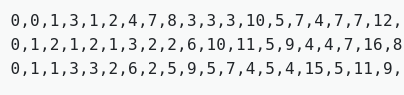
\includegraphics[width=0.5\textwidth]{../images/datos-artritis.png}
            \end{flushright}
        }
    \item<3-> Visualización
        \only<3>{
            \begin{flushright}
                \vspace{-3cm}
                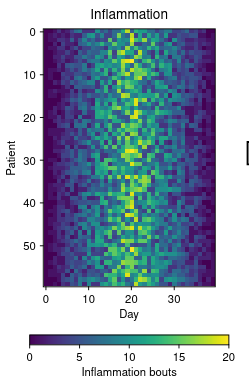
\includegraphics[width=0.3\textwidth]{../images/datos-artritis2.png}
            \end{flushright}
        }
    \item<4-> Estadística $\to$ Concluir!
\end{itemize}
\end{frame}
%%%%%%%%%%%%%%%%%%%%%%%%%%%%%%%%%%%%%%%%%%%%%%%%%%%%%%%
\begin{frame}\frametitle{Ej II: Pensamiento algorítmico}
Cómo salgo de esta sala? (avanzar un paso, girar)

\vspace{2cm}
\pause Y si solo sé girar a la derecha?

\end{frame}
%%%%%%%%%%%%%%%%%%%%%%%%%%%%%%%%%%%%%%%%%%%%%%%%%%%%%%%
\begin{frame}\frametitle{Ej II: Lo que hicimos}
    \begin{itemize}
        \item Considerar un pequeño conjunto de instrucciones
        \item Generar nuevas instrucciones más complejas {\color{gray}(como la célula!)}
        \item Combinar instrucciones para un objetivo
    \end{itemize}
\end{frame}
%%%%%%%%%%%%%%%%%%%%%%%%%%%%%%%%%%%%%%%%%%%%%%%%%%%%%%%
\section{Interacción con el PC}
%%%%%%%%%%%%%%%%%%%%%%%%%%%%%%%%%%%%%%%%%%%%%%%%%%%%%%%
\begin{frame}\frametitle{Sistemas operativos}
El OS coordina funcionamiento del computador. \pause
    \begin{itemize}
        \item<+-> Windows (MS-DOS)
        \item<+-> Mac OS (BSD Darwin)
        \item<+-> BSD (FreeBSD, OpenBSD)
        \item<+-> GNU/Linux (Debian, Ubuntu, Fedora, $\hdots$)
        \item<+-> Android
        \item<+-> iOS
        \item<+-> Symbian
        \item<+-> BeOS, Haiku
    \end{itemize}
\end{frame}
%%%%%%%%%%%%%%%%%%%%%%%%%%%%%%%%%%%%%%%%%%%%%%%%%%%%%%%
\begin{frame}\frametitle{Sistemas operativos}
    \begin{center}
        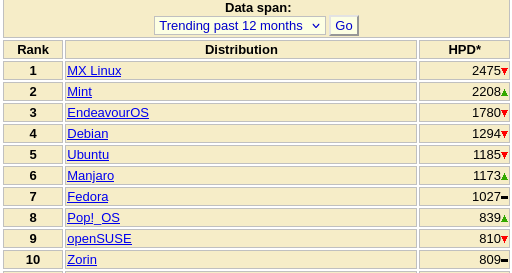
\includegraphics[width=0.5\textwidth]{../images/distrowatch.png}
    \end{center}
\end{frame}
%%%%%%%%%%%%%%%%%%%%%%%%%%%%%%%%%%%%%%%%%%%%%%%%%%%%%%%
%\begin{frame}\frametitle{Sistemas operativos}
%    \begin{columns}
%        \begin{column}{0.45\textwidth}
%        \begin{small}
%        \begin{table}
%            \renewcommand\arraystretch{1.4}\arrayrulecolor{LightSteelBlue3}
%            %\captionsetup{singlelinecheck=false, font=blue, labelfont=sc, labelsep=quad}
%
%            %\begin{minipage}{7cm}
%                %\caption*{}
%            %\end{minipage}
%            \vskip -1.5ex
%
%            \begin{tabular}{@{\,}r <{\hskip 2pt} !{\foo} >{\raggedright\arraybackslash}p{5cm}}
%            \addlinespace[1.5ex]
%            1956   & General Motors  \\
%            1960's & UNIX  \\
%            1977   & Apple \\
%            1981   & MS-DOS \\
%            1991   & Linux (GNU/Linux) \\
%            1995   & Windows 95 \\
%            2000   & Darwin (macOS) \\
%            2007   & iOS \\
%            2008   & Android
%            \end{tabular}
%        \end{table}
%        \end{small}
%        \end{column}
%        \begin{column}{0.5\textwidth}
%            \only<1>{
%                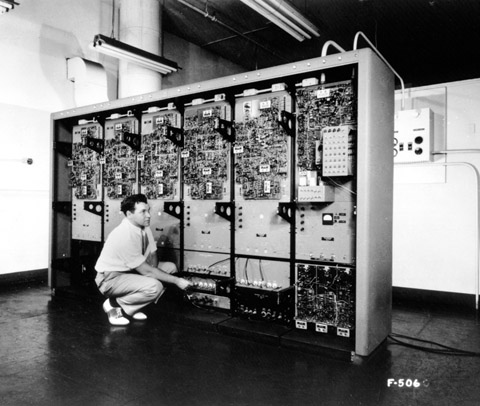
\includegraphics[width=\textwidth]{../images/os-gm.png}
%                GM para primer IBM }
%            \only<2>{
%                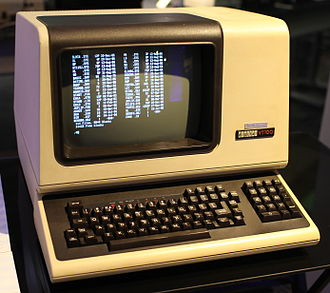
\includegraphics[width=0.9\textwidth]{../images/os-unix.png}
%                Terminal UNIX}
%            \only<3>{
%                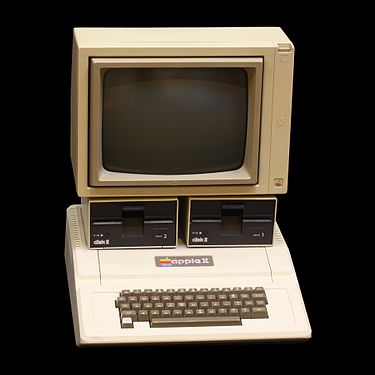
\includegraphics[width=0.8\textwidth]{../images/os-appleii.png}
%                Primer Apple ][}
%            \only<4>{
%                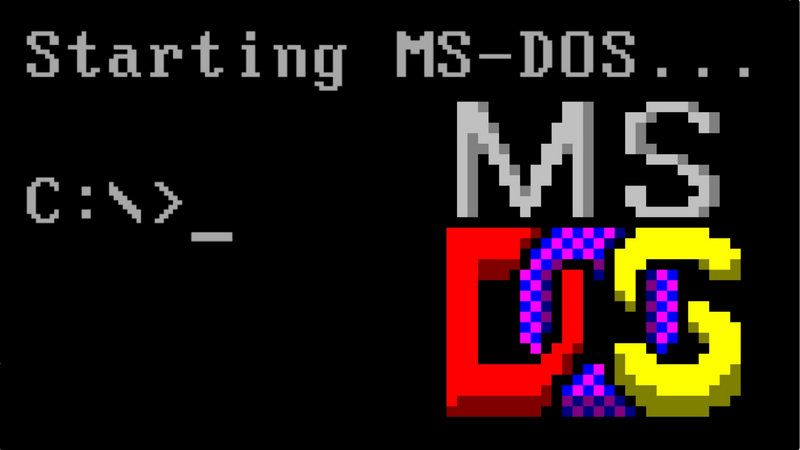
\includegraphics[width=\textwidth]{../images/os-msdos.png}
%                MSDOS (Microsoft)}
%            \only<5>{
%                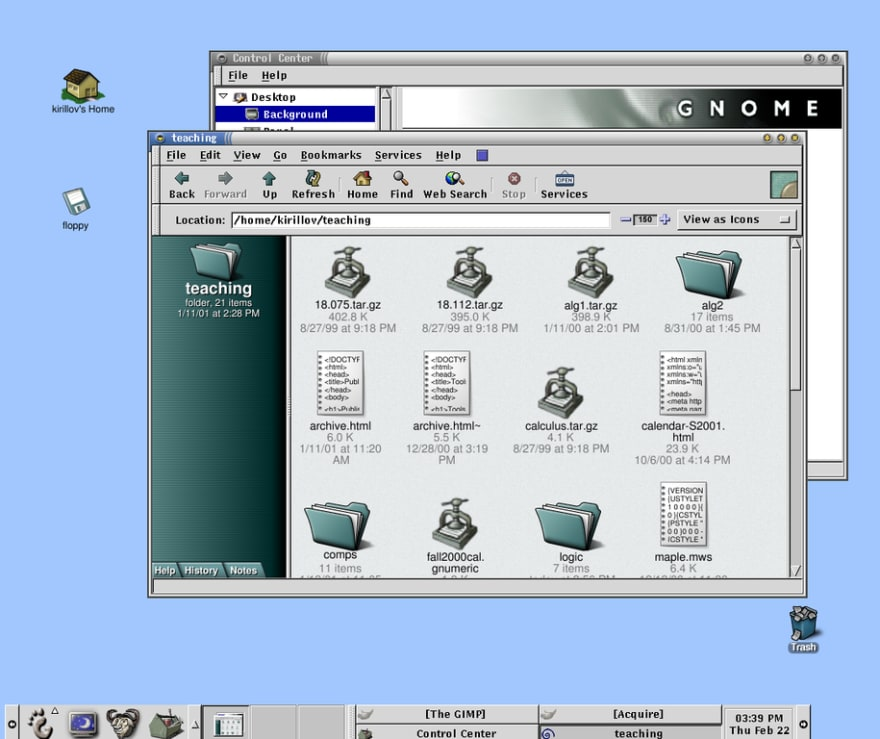
\includegraphics[width=\textwidth]{../images/os-linux.png}
%                Linux desktop}
%            \only<6>{
%                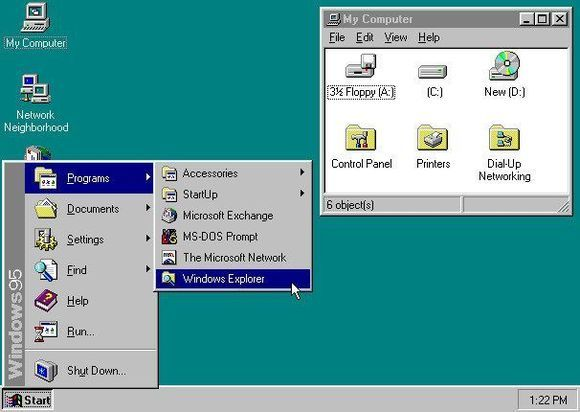
\includegraphics[width=\textwidth]{../images/os-windows95.png}
%                Escritorio \emph{moderno} (Win95) }
%            \only<7>{
%                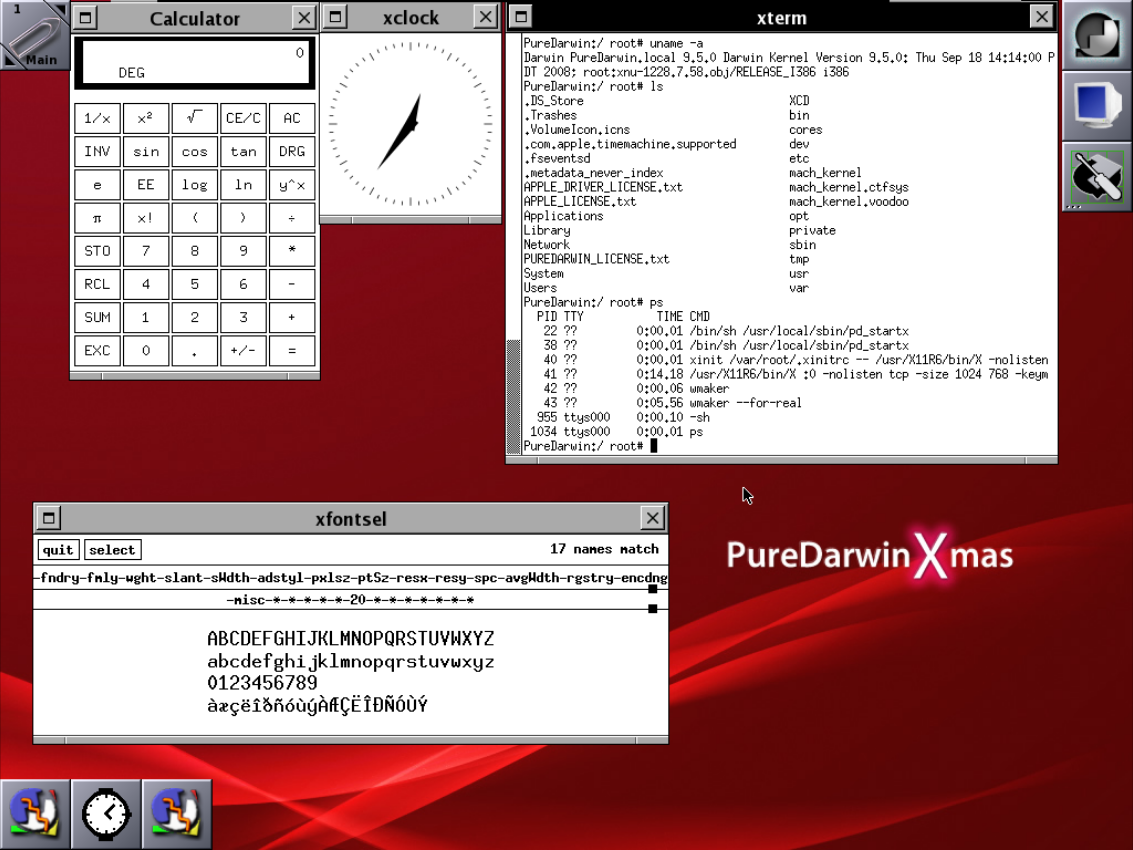
\includegraphics[width=\textwidth]{../images/os-darwin.png}
%                Bases de macOS}
%            \only<8>{
%                
\includegraphics[width=\textwidth]{../images/os-ios.png}
%                }
%            \only<9>{
%                
\includegraphics[width=0.8\textwidth]{../images/os-android.png}
%                }
%        \end{column}
%    \end{columns}
%\end{frame}
%%%%%%%%%%%%%%%%%%%%%%%%%%%%%%%%%%%%%%%%%%%%%%%%%%%%%%%
\section{La consola}
%%%%%%%%%%%%%%%%%%%%%%%%%%%%%%%%%%%%%%%%%%%%%%%%%%%%%%%
\begin{frame}\frametitle{Principio}
    \begin{itemize}
        \item La consola (Unix) es una forma de interacción con el PC
        \item Funciona a través de programas
        \item Las interfaces gráficas usan consola!
    \end{itemize}
    \begin{flushright}
        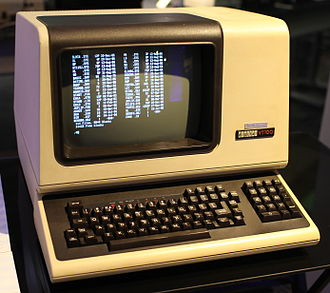
\includegraphics[width=0.4\textwidth]{../images/os-unix.png}
    \end{flushright}
\end{frame}
%%%%%%%%%%%%%%%%%%%%%%%%%%%%%%%%%%%%%%%%%%%%%%%%%%%%%%%
\begin{frame}\frametitle{La consola: Inicio}
La consola Bash en Linux permite interactuar con el PC\footnote{Se puede instalar en Windows con WSL, queda para ayudantía}

    \begin{center}
        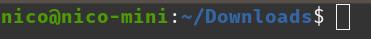
\includegraphics[width=0.6\textwidth]{../images/consola.png}
    \end{center}
\begin{itemize}
    \item \texttt{nico}: Usuario
    \item \texttt{nico-mini}: hostname, nombre de red del PC
    \item \texttt{\texttilde/Downloads}: Carpeta actual
    \item \texttt{\texttilde}: Carpeta 'home'
\end{itemize}
\end{frame}
%%%%%%%%%%%%%%%%%%%%%%%%%%%%%%%%%%%%%%%%%%%%%%%%%%%%%%%
\begin{frame}\frametitle{Sistema de archivos}
En Linux, los archivos funcionan como uno espera:
    \begin{itemize}
        \item Carpeta 1
            \begin{itemize}
                \item Archivo 1
                \item Archivo 2
            \end{itemize}
        \item Carpeta 2
            \begin{itemize}
                \item Carpeta 3
                \item Archivo 3
            \end{itemize}
        \item $\dots$
    \end{itemize}

\end{frame}
%%%%%%%%%%%%%%%%%%%%%%%%%%%%%%%%%%%%%%%%%%%%%%%%%%%%%%%
\begin{frame}\frametitle{Navegación básica en Bash}
    \begin{itemize}
        \item \texttt{ls}: Mostrar contenido de carpeta
        \item \texttt{cd}: Cambiar de directorio
        \item \texttt{mkdir}: Crear carpeta
        \item \texttt{rm}: Eliminar archivo o carpeta
        \item \texttt{cp}: Copiar archivo o carpeta
        \item \texttt{nano}: Editor de texto
        \item \texttt{cat}: Mostrar archivo
    \end{itemize}

\vspace{1cm} 
Pro-tip: Autocompletar con \texttt{tab}
\end{frame}
%%%%%%%%%%%%%%%%%%%%%%%%%%%%%%%%%%%%%%%%%%%%%%%%%%%%%%%
\begin{frame}[fragile]\frametitle{Concepto de programa}
Ver contenidos de 'Documents':

    $$ \texttt{\$ }\underbrace{\texttt{ls}}_\text{Comando}  \underbrace{Documents}_\text{Argumento} $$
\end{frame}
%%%%%%%%%%%%%%%%%%%%%%%%%%%%%%%%%%%%%%%%%%%%%%%%%%%%%%%
\begin{frame}\frametitle{Argumentos y opciones}
    
    $$ \texttt{\$ }\underbrace{\texttt{ls}}_\text{Comando} \quad \underbrace{\texttt{-l -a --color}}_\text{Opciones} \quad \underbrace{Documents}_\text{Argumento} $$

La más útil: \texttt{--help/-h}. 

\vspace{1cm}
\idea{Veamos...}
\end{frame}
%%%%%%%%%%%%%%%%%%%%%%%%%%%%%%%%%%%%%%%%%%%%%%%%%%%%%%%
\section{Compilación de código}
%%%%%%%%%%%%%%%%%%%%%%%%%%%%%%%%%%%%%%%%%%%%%%%%%%%%%%%
\begin{frame}[t]\frametitle{La compilación}
    \idea{Consiste en traducir nuestro lenguaje al del PC}

    \vspace{1cm}
    \begin{itemize}
        \item<+-> Lo que nosotros entendemos: Lenguaje
        \item<+-> Lo que entiende el computador: 
    
        100010101010110101011010110101011011010101011101010000
            
    \end{itemize}
\end{frame}
%%%%%%%%%%%%%%%%%%%%%%%%%%%%%%%%%%%%%%%%%%%%%%%%%%%%%%%
\begin{frame}[fragile]\frametitle{Ejemplo de compilación}
\begin{small}
    \begin{columns}[t]
        \begin{column}[b]{0.4\textwidth}
            Para humanos:
            \vspace{2.0cm}
            \begin{minted}{C}
#include <stdio.h>
   int main() {
   printf("Hello, World!\n");
   return 0;
            }
            \end{minted}

    \vfill
        \end{column}
        \begin{column}{0.01\textwidth}
            \rule{0.4pt}{6cm}

        \end{column}
        \begin{column}[b]{0.45\textwidth}
            Para PC: 
            \begin{minted}{gas}
    .file    "hello.c"
    .text
    .section .rodata
.LC0:
    .string  "Hello, World!"
    .text
    .globl   main
    .type    main, @function
main:
            \end{minted}

    \vfill
        \end{column}
    \end{columns}
\end{small}
\end{frame}
%%%%%%%%%%%%%%%%%%%%%%%%%%%%%%%%%%%%%%%%%%%%%%%%%%%%%%%
\begin{frame}\frametitle{El trabajo de compilación}
    \begin{enumerate}
        \item Procesar el archivo con código
        \item Generar símbolos de programas
        \item Juntar símbolos para generar programa
    \end{enumerate}

    \pause \begin{center}
        \begin{tabular}{c | c}
           Pros    &   Contras \\ \midrule
         \alertGreen{Eficiente} &   \alert{Inflexible}  \\
        \end{tabular}
    \end{center}

\pause Ejemplos de programas compilados: \texttt{ls, cd, }$\hdots$
\end{frame}
%%%%%%%%%%%%%%%%%%%%%%%%%%%%%%%%%%%%%%%%%%%%%%%%%%%%%%%
\begin{frame}\frametitle{Alternativa}
Lenguajes compilados son eficientes pero...
    \begin{itemize}
        \item Más complejos
        \item Requieren recompilar constantemente
    \end{itemize}

\vspace{1cm}
\pause Alternativa: \textbf{Lenguajes interpretados}

\pause
    \begin{itemize}
        \item Muchos subprogramas pre-compilados
        \item No se compila, se ejecuta secuencialmente (una línea a la vez)
        \item Permiten una consola interactiva
    \end{itemize}
\end{frame}
%%%%%%%%%%%%%%%%%%%%%%%%%%%%%%%%%%%%%%%%%%%%%%%%%%%%%%%
\begin{frame}\frametitle{Algunos ejemplos}
    \begin{columns}
        \begin{column}{0.45\textwidth}
            Compilados
            \begin{itemize}
                \item C/C++/C\#
                \item Java
                \item Rust
                \item Julia
            \end{itemize}
        \end{column}

        \begin{column}{0.45\textwidth}
            Interpretados
            \begin{itemize}
                \item Python
                \item R
                \item MATLAB
            \end{itemize}
        \end{column}
    \end{columns}
\end{frame}
%%%%%%%%%%%%%%%%%%%%%%%%%%%%%%%%%%%%%%%%%%%%%%%%%%%%%%%
\begin{frame}\frametitle{Ranking de lenguajes (2024)}
    \begin{center}
        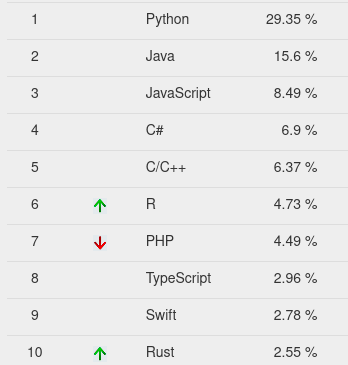
\includegraphics[width=0.4\textwidth]{../images/top-lenguajes.png}
    \end{center}
\end{frame}
%%%%%%%%%%%%%%%%%%%%%%%%%%%%%%%%%%%%%%%%%%%%%%%%%%%%%%%
\section{Python}
%%%%%%%%%%%%%%%%%%%%%%%%%%%%%%%%%%%%%%%%%%%%%%%%%%%%%%%
\begin{frame}\frametitle{Datos sobre Python}
    \begin{itemize}
        \item Lenguaje interpretado, orientado a objetos
        \item Creado en 1991 por Guido van Rossum
        \item Basado en C
        \item Librerías de IA: PyTorch, Keras, TensorFlow
        \item MUCHAS librerías científicas
        \item Ejecuta extensión \texttt{'.py'}
    \end{itemize}

\begin{block}{}
    \emph{[...] as a hobby project to keep himself busy during the Christmas holidays of 1989. }
\end{block}
\end{frame}
%%%%%%%%%%%%%%%%%%%%%%%%%%%%%%%%%%%%%%%%%%%%%%%%%%%%%%%
\begin{frame}\frametitle{Cómo usar Python}
    \begin{enumerate}
        \item<1-> Como programa
            \only<1>{
                \begin{flushright}
                    \texttt{nico@nico-pc:\texttilde/Codes\$ python test.py}
                \end{flushright}
            }
        \item<2-> Como consola interactiva
            \only<2>{
                \begin{flushright}
                    \texttt{nico@nico-pc:\texttilde/Codes\$ python} 
                    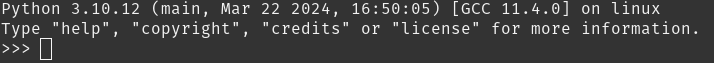
\includegraphics[width=0.9\textwidth]{../images/python-intepreter.png}
                \end{flushright}
            }
        \item<3-> \textbf{Jupyter/Collab/IDE (ayudantía)}
    \end{enumerate}

\vspace{1cm}
\pause\idea{Veamos la consola}
\end{frame}
%%%%%%%%%%%%%%%%%%%%%%%%%%%%%%%%%%%%%%%%%%%%%%%%%%%%%%%
\begin{frame}[t]\frametitle{Primeros códigos}
    \begin{itemize}
        \item Definición de variables (case sensitive)
            $$ > \underbrace{\texttt{a = 2}}_\text{Asignación \emph{siempre} de derecha a izquierda} $$
        \item Toda variable tiene un tipo 
            \begin{itemize}
                \item \texttt{> a = 2} : \hspace{0.3cm}\>\>\>\>\> 'a' es un 'int' (entero)
                \item \texttt{> a = 3.14}: \>\>\>\>\>'a' es un 'float' (punto flotante)
                \item \texttt{> a = "hola"}: 'a' es un 'string' (texto)
                \item \texttt{> a = True}: \>\>\> 'a' es un 'bool' (booleano)\footnote{esto tendrá sentido más adelante}
            \end{itemize}
        \item Se pueden dejar comentarios con \#
    \end{itemize}

\idea{Veamos en consola usando la función \texttt{type}}
\end{frame}
%%%%%%%%%%%%%%%%%%%%%%%%%%%%%%%%%%%%%%%%%%%%%%%%%%%%%%%
\begin{frame}\frametitle{Aritmética}
Cuál es el valor resultante de las siguientes operaciones? 

\vspace{1cm}
    \begin{itemize}
        \item \texttt{> a = 2+2}
        \item \texttt{> a = 2+2*2}
        \item \texttt{> a = 2/2*2}
        \item \texttt{> a = 2**2}   \textcolor{gray}{(elevado)}
        \item \texttt{> a = 'ho' + 'la'}
    \end{itemize}

\idea{Ojo: división entre enteros da un 'float'}

\end{frame}
%%%%%%%%%%%%%%%%%%%%%%%%%%%%%%%%%%%%%%%%%%%%%%%%%%%%%%%
\begin{frame}\frametitle{Nota sobre la división}
La división se entiende como aplicada exclusivamente al número precedente. Eso implica lo siguiente: 
    \begin{itemize}
        \item \texttt{2/2} es $\frac 2 2$
        \item \texttt{2/2*2} es $\left(\frac 2 2\right) \times 2$
        \item \texttt{2/2/2} es $\frac{\left(\frac 2 2\right)}{2}= \frac{2}{2\times 2}$
    \end{itemize}

\pause \idea{Es más fácil imaginar $a/b$ como $a \times b^{-1}$}
\end{frame}
%%%%%%%%%%%%%%%%%%%%%%%%%%%%%%%%%%%%%%%%%%%%%%%%%%%%%%%
\begin{frame}\frametitle{Álgebra booleana}
    Keywords importantes: 
    \begin{itemize}
        \item \texttt{and}, \texttt{or}, \texttt{not}
        \item \texttt{==}, \texttt{<=}, \texttt{>=}, \texttt{<}, \texttt{>}
    \end{itemize}

En términos de precedencia, \alertBlue{\texttt{and}} es un producto y \alertBlue{\texttt{or}} es una suma: 

$$ \texttt{a and b or c} = (\texttt{a and b}) \texttt{ or } c $$

Notar que el resultado es siempre otro booleano.
\end{frame}
%%%%%%%%%%%%%%%%%%%%%%%%%%%%%%%%%%%%%%%%%%%%%%%%%%%%%%%
\begin{frame}\frametitle{Recap}
    \begin{itemize}
        \item Qué es programar, pensamiento algorítmico
        \item Sistemas operativos
        \item Podemos interactuar con el PC a través de la consola (Unix)
        \item Concepto de compilación
        \item Python: lenguaje interpretado, orientado a objetos
        \item Usamos la consola interactiva de Python
        \item Tipos de variables: int, float, bool, string
        \item Operaciones entre variables, aritmética y álgebra

    \end{itemize}
\end{frame}
%%%%%%%%%%%%%%%%%%%%%%%%%%%%%%%%%%%%%%%%%%%%%%%%%%%%%%%

%%%%%%%%%%%%%%%%%%%%%%%%%%%%%%%%%%%%%%%%%%%%%%%%%%%%%%%
\begin{frame}
    \maketitle
\end{frame}
%%%%%%%%%%%%%%%%%%%%%%%%%%%%%%%%%%%%%%%%%%%%%%%%%%%%%%%

\end{document}
